\documentclass{article}
\title{CUDA Parallel Programming\\Homework 3}
\usepackage{graphicx}
\usepackage[UTF8]{ctex}
\usepackage{hyperref}
\usepackage{amsmath}
\CTEXoptions[today=old]
\author{40647007S 朱健愷}

\begin{document}
	\maketitle
	\section{Source codes}
	\subsection{File Layout}
	\begin{itemize}
		\item laplaceTex/laplace.cu - First problem's main code containing both CPU and GPU code without using texture memory
		\item laplaceTex/laplaceTex.cu - First problem's main code containing both CPU and GPU code using texture memory
		\item laplaceTex3D/laplace.cu - Second problem's main code containing both CPU and GPU code
		\item laplaceTex3D/poisson\textunderscore{pc}.cu - Third problem's main code containing both CPU and GPU code
		\item Makefile - Script to auto generate executable from code
		\item laplaceTex/experiment.sh - Script to auto generate results of solving first problem's 2D Laplace equation using different block size
		\item laplaceTex3D/experiment.sh - Script to auto generate results of solving second's 3D Laplace equation and third problem's 3D Poisson equation using different L size
		\item laplaceTex/result/block\textunderscore*/ - Output result of solving first problem's 2D Laplace equation with different block size, the suffix represent the block size. In this directory contains initial phi data, phi data calculated by CPU, GPU, and statistical result of solving 2D laplace equation without using texture memory.
		\item laplaceTex/result/Tex\textunderscore{block}\textunderscore*/ - Output result of solving first problem's 2D Laplace equation with different block size, the suffix represent the block size. In this directory contains initial phi data, phi data calculated by CPU, GPU, and statistical result of solving 2D laplace eqaution using texture memory.
		\item laplaceTex3D/result/Laplace\textunderscore3D - Output result of solving second problem's 3D Laplace equation using $4\times4\times4$ lattice, the suffix represent the block size. In this directory contains initial phi data, phi data calculated by CPU, GPU, and statistical result of solving 3D laplace eqaution.
		\item laplaceTex3D/result/Poisson\textunderscore3D\textunderscore* - Output result of solving third problem's 3D poisson equation using $L=8, 16, 32, 64$, the suffix represent the lattice size in each dimension. In this directory contains initial phi data, phi data calculated by CPU, GPU, and statistical result of solving 3D poisson eqaution.
		\item notebook/*.png - Plots concluding output result
	\end{itemize}
	
	
	\subsection{Usage}
	Make code in both laplaceTex/ and laplaceTex3D/ directories
	Run the experiment.sh script in both laplaceTex/ and laplaceTex3D/ directories 
	
	\begin{verbatim}
	cd laplaceTex
	make
	sh experiment.sh
	cd ../laplaceTex3D
	make
	sh experiment.sh
	\end{verbatim}
	
	And it will produce three problems statistical result using different.
	\section{Formula}
	\subsection{Second problem}
	For second problem, we need to extend the laplace operator defined in discrete grid from 2D into 3D. The laplace operator in 2D case is
	
	\begin{equation}
	\nabla^2\phi=\frac{\partial^2\phi}{\partial{x}^2} + \frac{\partial^2\phi}{\partial{y}^2}
	\end{equation}
	
	Extend it to 3D case yield

	\begin{equation}
	\nabla^2\phi=\frac{\partial^2\phi}{\partial{x}^2} + \frac{\partial^2\phi}{\partial{y}^2} + \frac{\partial^2\phi}{\partial{z}^2}
	\end{equation}

	The discrete laplace equation in 2D can be rewrite to

	\begin{equation}
	\frac{\phi(x+a, y)+\phi(x-a, y)-2\phi(x, y)}{a^2}+\frac{\phi(x, y+a)+\phi(x, y-a)-2\phi(x, y)}{a^2}\equiv{D\phi}=\rho
	\end{equation}
	
	Extending to 3D case is
	
	\begin{equation}
		\begin{aligned}
		\frac{\phi(x+a, y, z)+\phi(x-a, y, z)-2\phi(x, y, z)}{a^2}+\frac{\phi(x, y+a, z)+\phi(x, y-a, z)-2\phi(x, y, z)}{a^2}+\\\frac{\phi(x, y, z+a)+\phi(x, y, z-a)-2\phi(x, y, z)}{a^2}\equiv{D\phi}=\rho
		\label{eq:ThreeD_Laplace}
		\end{aligned}
	\end{equation}
	
	In Laplace equation, $\rho$ is $0$, and unit of grid is $a=1$, so rearanging above equation yield
	
	\begin{equation}
	\phi(x, y, z)=\frac{\phi(x+a, y, z)+\phi(x-a, y, z)+\phi(x, y+a, z)+\phi(x, y-a, z)+\phi(x, y, z+a)+\phi(x, y, z-a)}{6}
	\end{equation}

	Using above equation to update the field with boundary condition specified, we can solve the Laplace equation on a 3D lattice.
	
	\subsection{Third problem}
	The Poisson equation is similar to Laplace equation, except that it has a point charge $q=1$ defined at cube center $(\frac{L}{2}, \frac{L}{2}, \frac{L}{2})$.
	
	Deriving from previous part we know that at cube center grid, the $\rho$ value is 1, using (\ref{eq:ThreeD_Laplace}) equation and rearanging it yield
	
	\begin{equation}
		\phi(x, y, z)=(\phi(x+a, y, z)+\phi(x-a, y, z)+\phi(x, y+a, z)+\phi(x, y-a, z)+\phi(x, y, z+a)+\phi(x, y, z-a) - 1)/6
	\end{equation}

	And at the other grid, the $\rho$ value is 0, so use original (\ref{eq:ThreeD_Laplace}) equation is enough.
	
	Concluding above, at the cube center grid $(\frac{L}{2}, \frac{L}{2}, \frac{L}{2})$, we solve Poisson equation with $\rho=1$, and at the other grid, we solve Laplace equation as usual.
	
	\section{Result}
	\subsection{Experiment environment}
	I ran my code on workstation provided in course, below is the Setup of workstation
	\begin{itemize}
		\item Operating system: Linux version 4.19.172 (root@twcp1)\\(gcc version 6.3.0 20170516 (Debian 6.3.0-18+deb9u1))
		\item CPU: Intel(R) Core(TM) i7-4790 CPU @ 3.60GHz
		\item GPU: Nvidia GTX 1060 6GB
		\item Memory: 32GB 
	\end{itemize}
	\subsection{Performance}
	\subsubsection{First problem}
	\newpage
	Below two figure and lines showed GPU without using texture memory, GPU using texture memory and CPU performance
	\begin{figure}
		\centering
		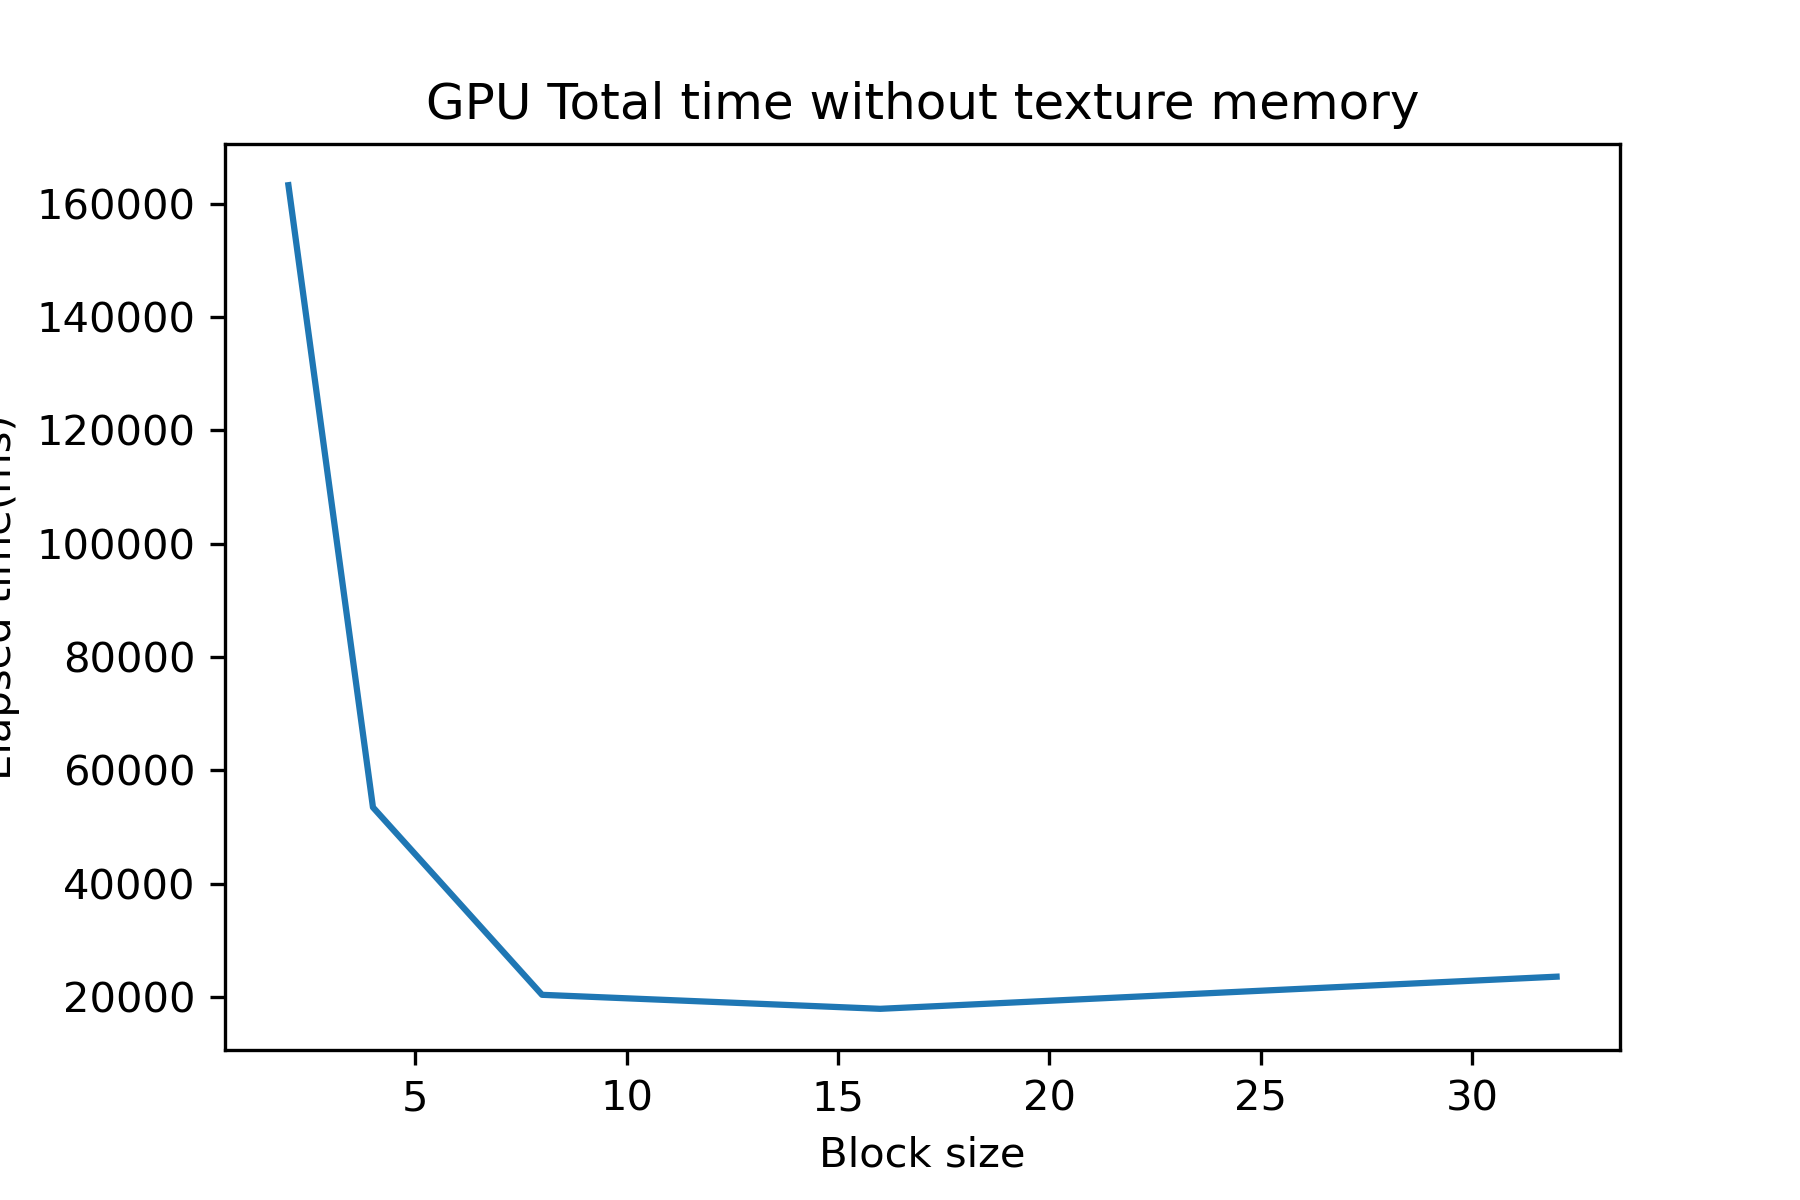
\includegraphics[width=\linewidth]{notebook/gpu_total_time}
	\end{figure}
	\begin{figure}[hb!]
		\centering
		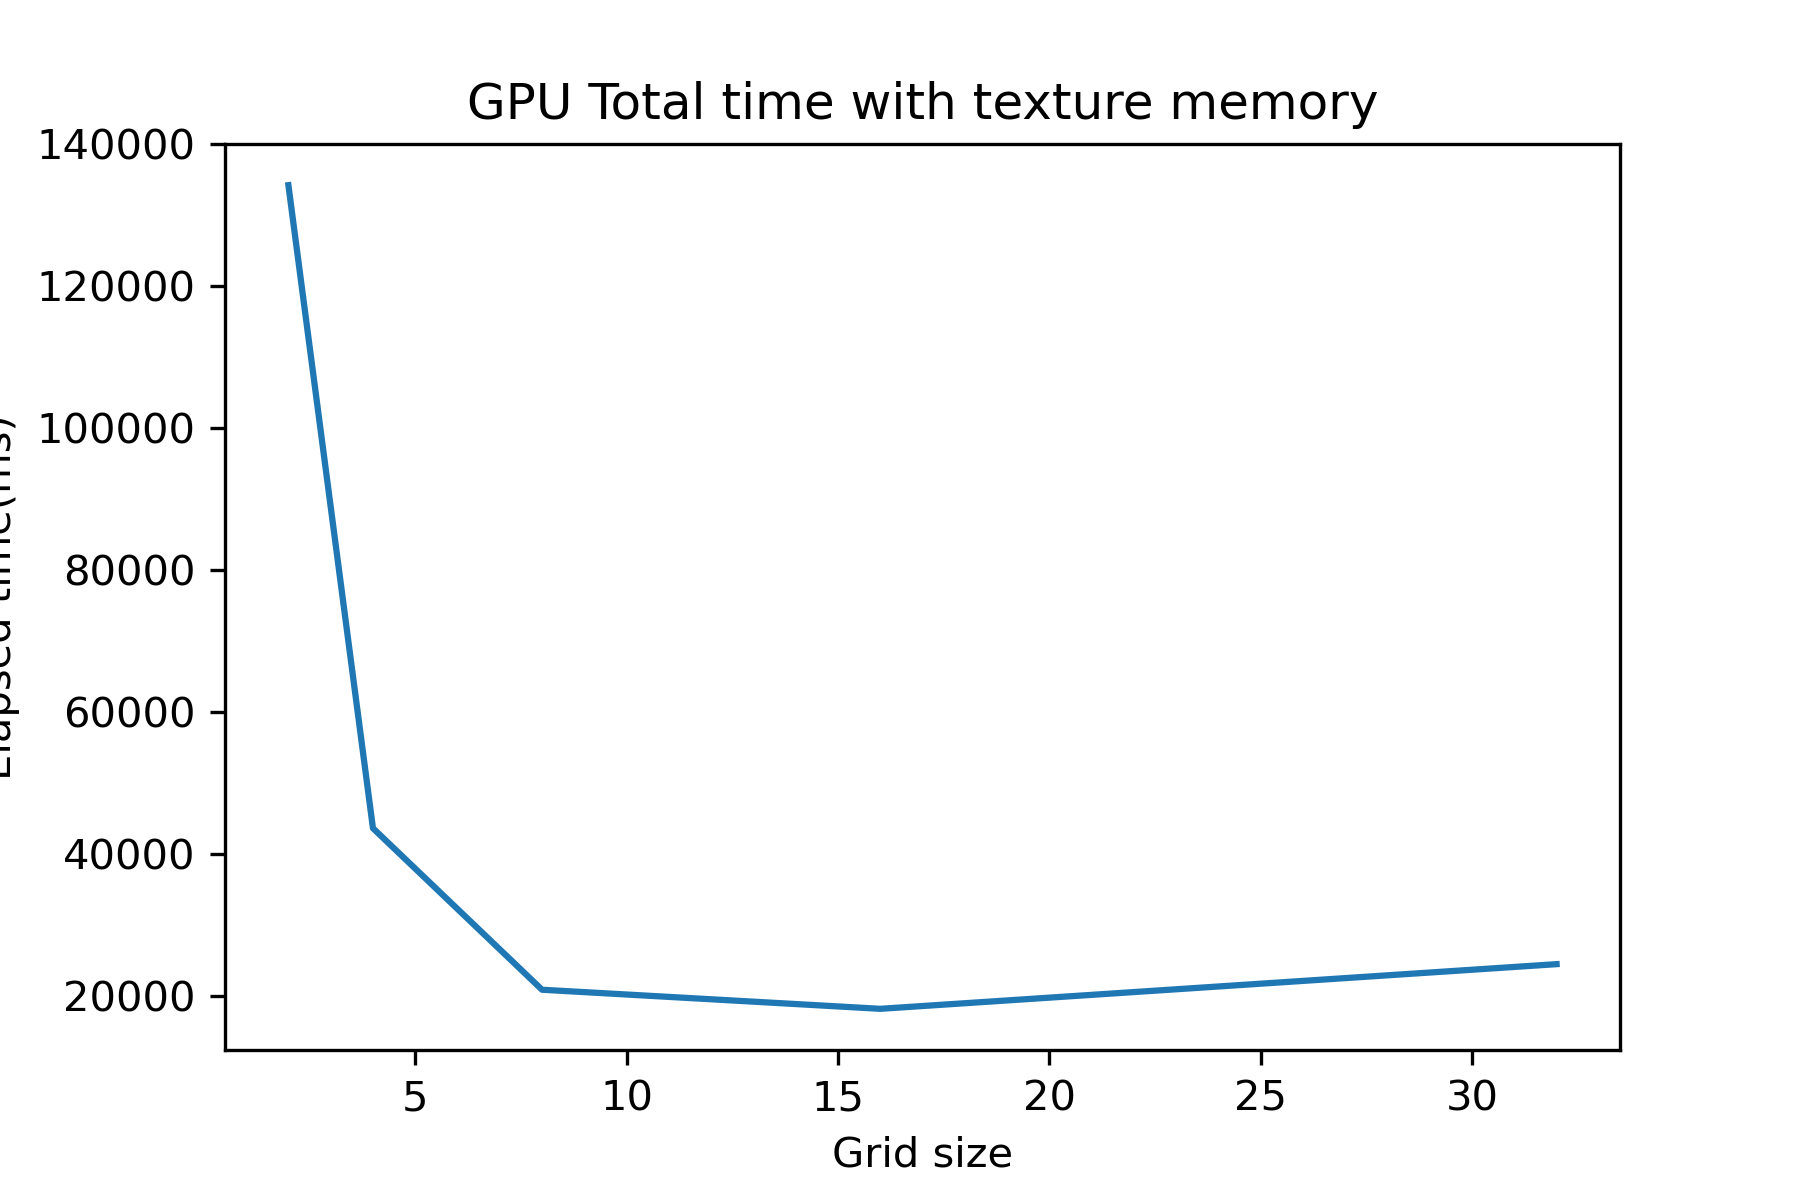
\includegraphics[width=\linewidth]{notebook/gpu_total_time_texture}
	\end{figure}

	CPU total time is 251365.921875, which is worse than any setup showed above.
	\subsubsection{Second problem}
	Using "diff" command, it showed that the result of GPU comparing to that of CPU is the same. Using (\ref{eq:ThreeD_Laplace}) to inspect every grid which were not in boundary showed that they correspond to the Laplace equation.

	\subsubsection{Third problem}
	We can see that the larger the grid size, the more each grid's potential magnitude approach to $\frac{1}{r}$ proportion where $r=\sqrt{(x-x_0)^2+(y-y_0)^2+(z-z_0)^2}$.

	\subsubsection{Observation}
	We can observe that the performance of small block size setup in both with texture memory usage and without it yield the worse performance in my experiment. This may because of when we do parallel reduction, we usually need many threads in block in order to collect each block's difference, and then gather the result using CPU. So the block size do affect the performance a lot.
	
	By comparing the statistical results of solving 2D Laplace equation using texture memory and without using it, I observed that in small block size setup, the one using texture memory have better performance than the one without using it. But in large block size setup, the one using texture memory have worse performance than the one without using it. 
	
	Same as the observation I observed in the previous assignment, the performance increase until block size increased to some extent. 
	
	\section{Discussion}
	After conducting experiment, I'm curious about how texture memory does really speed up the calculation, so I've searched some information about it, the result told me that the texture memory is essentially a global memory, but because of special hardware acceleration, it is faster in filtering operations like linear floating point interpolation, and the cache it used is optimised for spatial locality (in the coordinate system of the texture) and not locality in memory.
	
	I thought that because its cache design is optimised for spatial locality but not locality in memory, in this application it should have better performance in all case against that without using texture memory because in all operation we perform, we use the coordinate positioning (which I thought is also a kind of spatial positioning), so the speed up should be fully utilized. But after thinking it more profound, I thought that the characteristic of cache may not be fully utilized because we were doing the write once read once operations, but not write once read many times operations, so cache miss may happens more often than we expect, which I thought that this can explain the solving laplace equation with texture memory is slower in large block size setup case than the one without texture memory.
	
	\section{Reference}
	\href{https://stackoverflow.com/questions/8767059/texture-memory-in-cuda-concept-and-simple-example-to-demonstrate-performance}{Texture memory discussion in stackoverflow}
	
	\href{https://materials.prace-ri.eu/448/3/ISPGC15lect3.pdf}{Introduction to Scientific Programming using GPGPU and CUDA
in 21th page}
\end{document}